\documentclass{beamer}

\usepackage{minted}
\usepackage{pgf}
\usepackage[utf8]{inputenc}
\usepackage{mdframed}

\BeforeBeginEnvironment{minted}{\begin{mdframed}}
\AfterEndEnvironment{minted}{\end{mdframed}}

\title{Applying FP Patterns}
\author{Markus Hauck (@markus1189)}

\date{Scala Enthusiasts Rhein Main, 2017}
\subject{Computer Science}
\usetheme{codecentric}

\renewcommand\texttt[1]{\mintinline{scala}/#1/}

\usemintedstyle{fruity}

\begin{document}
\frame{\titlepage}

\section{Intro}
\label{sec:intro}

\begin{frame}
  \frametitle{Introduction}
  \begin{itemize}
  \item FP becomes more popular
  \item there are many useful patterns
    \begin{itemize}
    \item Monoids
    \item Better Error Handling
    \end{itemize}
  \end{itemize}
\end{frame}

\section{Composition}

\begin{frame}
  \frametitle{Lego vs Duplo}
  \begin{center}
    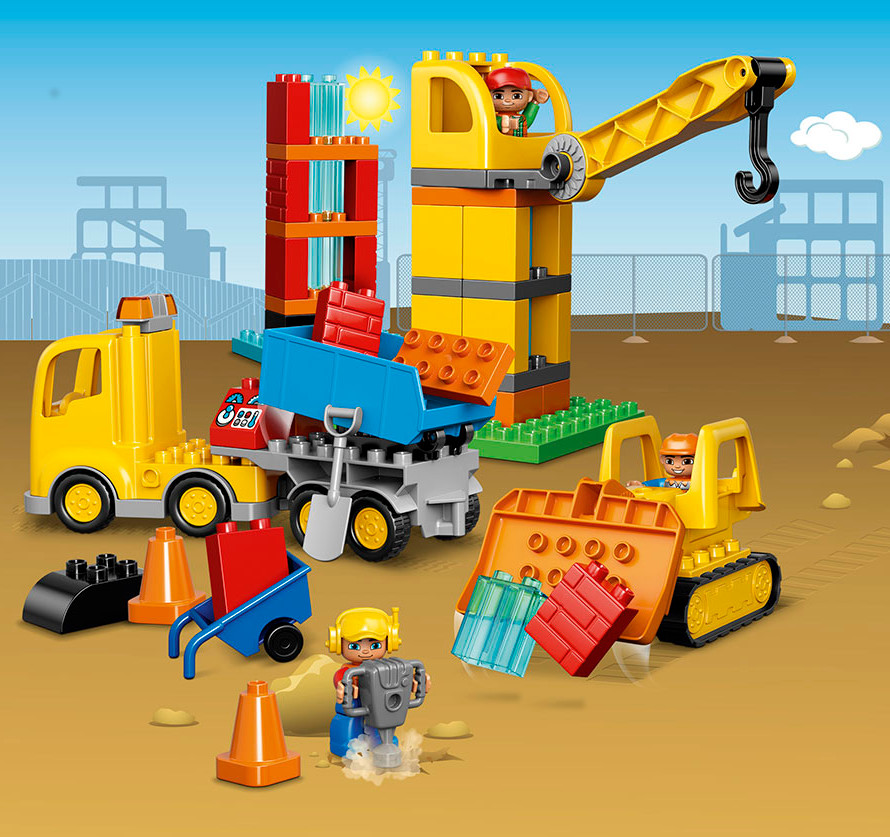
\includegraphics[width=0.48\textwidth]{../images/duplo-construction.jpg}
    \hspace{1mm}
    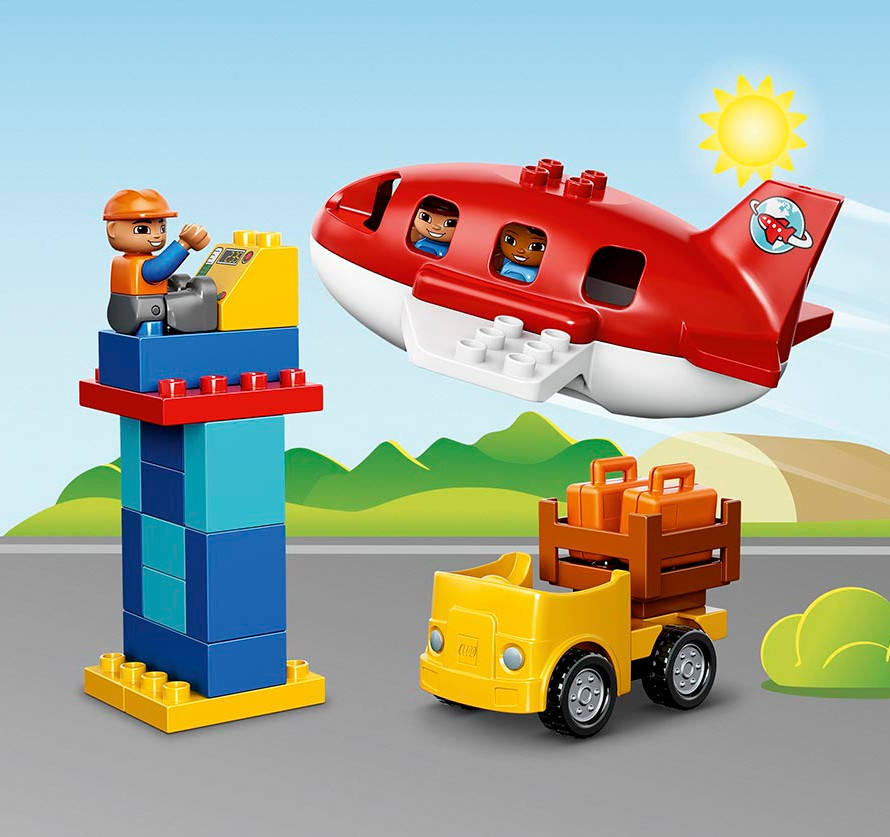
\includegraphics[width=0.48\textwidth]{../images/duplo-airport.jpg}
  \end{center}
  \vfill
  \begin{center}
    {\tiny pictures from \url{shop.lego.com}}
  \end{center}
\end{frame}

\begin{frame}
  \frametitle{Lego vs Duplo}
  \begin{center}
    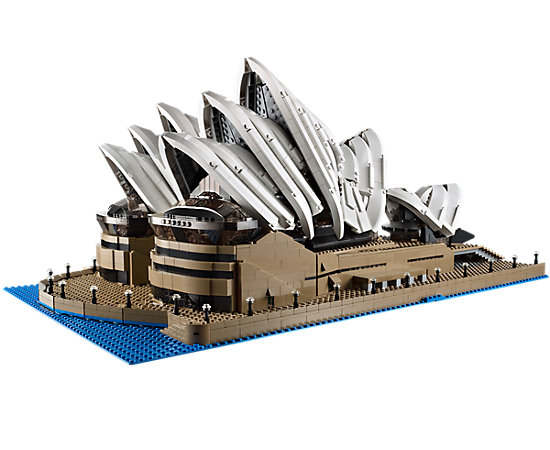
\includegraphics[width=0.49\textwidth]{../images/lego-sydney-opera.jpg}
    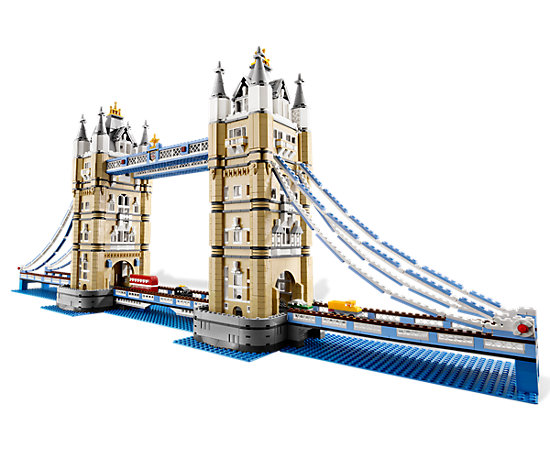
\includegraphics[width=0.49\textwidth]{../images/lego-tower-bridge.jpg}
  \end{center}
  \vfill
  \begin{center}
    {\tiny pictures from \url{shop.lego.com}}
  \end{center}
\end{frame}

\begin{frame}
  \frametitle{Lego vs Duplo}
  \begin{itemize}
  \item<1-> \textbf{Duplo} favours large specialized building blocks
    \begin{itemize}
    \item<1-> blocks tend to be too big
    \item<1-> limited reuse
    \end{itemize}
  \item<2-> \textbf{Lego} focuses on small composable building blocks
    \begin{itemize}
    \item<2-> blocks can conveniently be reused for other purposes
    \item<2-> limited use of specialized building blocks
    \end{itemize}
  \end{itemize}
  \onslide<3->
  \vfill
  \begin{center}
    \textbf{OO} tends to be like \textbf{Duplo}, \textbf{FP} tends to
    be like \textbf{Lego}
  \end{center}

\end{frame}

\section{Monoids}

\begin{frame}
  \frametitle{Monoids}
  \begin{itemize}
  \item intuition: ``combine stuff''
  \item you can create values from thin air via \texttt{Monoid.empty}
  \item combine two values via \texttt{Monoid.combine} / \texttt{|+|}
  \item additionally: \textit{laws} (don't write buggy implementations)
  \end{itemize}
\end{frame}

\begin{frame}[fragile]
  \frametitle{Monoid Laws}
\begin{minted}{scala}
// 1) left identity
empty |+| x === x

// 2) right identity
x |+| empty === x

// 3) associative
x |+| (y |+| z) === (x |+| y) |+| z
\end{minted}
\end{frame}

\begin{frame}[fragile]
  \frametitle{Monoid Typeclass}
\begin{minted}{scala}
trait Monoid[A] {
  def empty: A
  def combine(lhs: A, rhs: A): A
  // infix operator: |+|
}

implicit val plus: Monoid[Int] = new Monoid[Int] {
  def empty: Int = 0
  def combine(lhs: Int, rhs: Int): Int = lhs + rhs
}

object Monoid {
  def apply[A:Monoid]: Monoid[A] = implicitly
}
\end{minted}
\end{frame}

\begin{frame}[fragile]
  \frametitle{Using Our Monoid}
\begin{minted}{text}
> Monoid[Int].empty
0
> Monoid[Int].combine(1,2)
3
> 1 |+| 2
3
> 42 |+| Monoid[Int].empty
42
> List(1,2,3).foldLeft(Monoid[Int].empty)(_ |+| _)
6
\end{minted}
\end{frame}

\begin{frame}
  \frametitle{More Monoids}
  \begin{itemize}
  \item \texttt{Monoid} instance not unique: addition / multiplication / min / max
  \item most collections are \texttt{Monoid}s: \texttt{List} / \texttt{Vector} / \texttt{Set}
  \item let's see some more examples
  \end{itemize}
\end{frame}

\begin{frame}[fragile,fragile]
  \frametitle{Monoid Zoo}
  \begin{tabular}{p{5cm} l}
    \only<1->{\texttt{List[A]} & is a \texttt{Monoid} \\}
    \only<2->{\texttt{A => B} & if \texttt{B} is a \texttt{Monoid} \\}
    \only<3->{\texttt{(A,B)} & if \texttt{A} \textbf{and} \texttt{B} are \texttt{Monoid}s \\}
    \only<4->{\texttt{Future[A]} & if \texttt{A} is a \texttt{Monoid} \\}
    \only<5->{\texttt{Map[A,B]} & if \texttt{B} is a \texttt{Monoid}}
  \end{tabular}
  \onslide<6->
\begin{minted}{scala}
val m1 = Map("as" -> 21, "bs" -> 4)
val m2 = Map("as" -> 21, "cs" -> 2)
m1 |+| m2
//  Map("as" -> 42, "bs" -> 4, "cs" -> 2)
\end{minted}
\end{frame}

\begin{frame}[fragile]
  \frametitle{Monoids Compose (Lego Principle)}
  \onslide<1->
\begin{minted}{scala}
Config => A
\end{minted}
  \onslide<2->
\begin{minted}{scala}
Config => Future[A]
\end{minted}
  \onslide<3->
\begin{minted}{scala}
Config => Future[Map[String,A]]
\end{minted}
  \onslide<4->
\begin{minted}{scala}
Config => Future[Map[String,(A,B)]]
\end{minted}
  \onslide<5->
\begin{minted}{scala}
Config => Future[Map[String,(A,Option[B])]]
\end{minted}
  \onslide<6->
\begin{minted}{scala}
Config => Future[Map[String,(Set[A],Option[B])]]
\end{minted}
\end{frame}

\begin{frame}
  \begin{center}
    
\includegraphics[width=0.6\textwidth]{../images/disapproval.jpg}
  \end{center}
  \begin{center}
    {\large I thought this was about \textbf{applying} patterns!}
  \end{center}
\end{frame}

\begin{frame}
  \begin{center}
    
\includegraphics[width=0.3\textwidth]{../images/spark-logo-trademark.png}
  \end{center}

  \begin{itemize}
  \item analysis of a potentially huge text
  \item calculate metrics over text
    \begin{itemize}
    \item word count
    \item char count
    \item min/max word length
    \item avg word length
    \item \dots (be flexible)
    \end{itemize}
  \item \textbf{goal}: single traversal $\leftrightarrow$ \textbf{easy} composition
  \end{itemize}
\end{frame}

\begin{frame}[fragile]
  \frametitle{RDDs and Folds}
\begin{minted}{scala}
abstract class RDD[T] {
  /**
   * Aggregate the elements of each partition,
   * and then the results for all the partitions,
   * using a given associative function and a
   * neutral "zero value".
   */
  def fold(zeroValue: T)(op: (T, T) => T): T
}
\end{minted}
\end{frame}

\begin{frame}[fragile]
  \frametitle{Monoidal RDDs}
\begin{minted}{scala}
implicit class MonoidRDD[T](val rdd: RDD[T]) {

  // avoid conflicts with fold/reduce etc
  def combine(implicit M: Monoid[T]): T =
    rdd.fold(M.empty)(M.combine(_,_))

}
\end{minted}
\end{frame}

\begin{frame}[fragile,fragile]
  \frametitle{The Program}
\begin{minted}{scala}
val sc: SparkContext = ???
val file: String = ???

val data = sc.textFile(file).  // read the file
  flatMap(_.split("""\W+""")). // split into words
  map(expand)                  // action!

def expand(w: String) = (1, w.length, Map(w -> 1))

val (words,chars,wordMap) = data.combine
\end{minted}
\end{frame}

\begin{frame}[fragile]
  \frametitle{Running this program}
\begin{minted}{text}
Scala Meetup: Rhein-Main Scala Enthusiasts
\end{minted}
  \onslide<2->
\begin{minted}{scala}
Seq("Scala","Meetup","Rhein","Main","Scala", ...)
\end{minted}
  \onslide<3->
\begin{minted}{scala}
Seq( // expand(w: String) = (1,w.length,Map(w->1))
  (1, 5, Map("Scala" -> 1)),
  (1, 6, Map("Meetup" -> 1)),
  (1, 5, Map("Rhein" -> 1)),
  (1, 4, Map("Main" -> 1)),
  // ...
)
\end{minted}
  \onslide<4->
\begin{minted}{scala}
(6,36,Map("Scala" -> 2,"Meetup" -> 1,"Rhein" -> 1,...))
\end{minted}
\end{frame}

\begin{frame}[fragile]
  \frametitle{Easy Extension}
\begin{minted}{scala}
val data: RDD[String] = ??? // as before

def expand(w: String) = (
  1,
  Max(w.length),          // max word length
  Min(w.length),          // min word length
  Map(w.length -> Set(w)) // words by count
)
val (count,max,min,byCount) = data.combine
\end{minted}
\end{frame}

\begin{frame}[fragile]
  \frametitle{The new program}
\begin{minted}{text}
Scala Meetup: Rhein-Main Scala Enthusiasts
\end{minted}
  \onslide<2->
\begin{minted}{scala}
Seq("Scala","Meetup","Rhein","Main","Scala", ...)
\end{minted}
  \onslide<3->
\begin{minted}{scala}
Seq(
  (1, Max(5), Min(5), Map(5 -> Set("Scala"))),
  (1, Max(6), Min(6), Map(6 -> Set("Meetup"))),
  (1, Max(5), Min(5), Map(5 -> Set("Rhein"))),
  (1, Max(4), Min(4), Map(4 -> Set("Main"))),
  (1, Max(5), Min(5), Map(5 -> Set("Scala"))),
  // ...
)
\end{minted}
  \onslide<4->
\begin{minted}{scala}
(6,Max(11),Min(4),Map(5->Set("Scala","Rhein"),...))
\end{minted}
\end{frame}

\begin{frame}
  \frametitle{More Monoid Tricks}
  \begin{itemize}
  \item ``filter'' values via \texttt{mempty} value
  \item map + reduce == two phase computation via monoids
  \item finger trees, choose Monoid, get random access list / queue / \dots
  \item Monoids Theme and Variations (Functional Pearl)
  \end{itemize}
\end{frame}

\section{Errors}
\label{sec:exceptions-and-errors}

\begin{frame}
  \begin{center}
    {\Huge Part Two: Errors}
  \end{center}
\end{frame}

\begin{frame}
  \frametitle{The Traditional Way}
  \begin{itemize}
  \item Java style: \texttt{try}/\texttt{catch}/\texttt{finally}
  \item \textit{checked} exceptions
    \begin{itemize}
    \item compiler help
    \item reduce return value checking
    \end{itemize}
  \item \textit{unchecked} exceptions
    \begin{itemize}
    \item only visible via docs, if documented at all
    \item the ``way to go'' in Java?
    \end{itemize}
  \item errors? return \texttt{null} / custom classes
  \end{itemize}
\end{frame}

\begin{frame}
  \frametitle{The Functional Way}
  \begin{itemize}
  \item Scala: only \textit{unchecked} exceptions
  \item but: \texttt{throw} and \texttt{catch} discouraged in FP anyway
  \item FP:\@ type system + first class values
  \end{itemize}
\end{frame}

\begin{frame}[fragile]
  \frametitle{Out Of The Box}
  \begin{itemize}
  \item \texttt{Either} / \texttt{Try}
    \begin{itemize}
    \item \texttt{Either} unbiased (before 2.12)
    \item \texttt{Try} not a lawful monad\dots
    \end{itemize}
  \item get the most by using a FP library
  \end{itemize}
\end{frame}

\begin{frame}[fragile]
  \frametitle{Try and Catch}
\begin{minted}{scala}
def convert(is: String*): List[Int] =
  is.map(_.toInt).toList
\end{minted}

\begin{minted}{scala}
convert("1","2","3","Hello World!","5")
\end{minted}
\begin{minted}[fontsize=\tiny]{text}
java.lang.NumberFormatException: For input string: "Hello World"
  at java.lang.NumberFormatException.forInputString(NumberFormatException.java:65)
  at java.lang.Integer.parseInt(Integer.java:580)
  at java.lang.Integer.parseInt(Integer.java:615)
  ...
\end{minted}
\end{frame}

\begin{frame}[fragile]
  \frametitle{Try and Catch: Not Compositonal}
\begin{minted}{scala}
try {
  convert("1","2","3","Hello World!","5")
} catch {
  case e: NumberFormatException => println("Oops")
}
\end{minted}
  \begin{itemize}
  \item type says nothing about errors
  \item only one option: fail fast
  \item what about getting \textit{all} errors or non-fatal warnings
  \item problem is that \texttt{try}/\texttt{catch} does not compose
    (Duplo)
  \end{itemize}
\end{frame}

\begin{frame}[fragile]
  \frametitle{Example Time}
  \begin{itemize}
  \item password validation
  \item constraints:
    \begin{itemize}
    \item length $\geq$ 8
    \item contains at least one number
    \item contains no spaces
    \item contains at least one upper char
    \end{itemize}
  \end{itemize}
\end{frame}

\begin{frame}[fragile]
  \frametitle{Validating Passwords}
\begin{minted}{scala}
sealed trait LoginError
case object PwTooShort extends LoginError
case object PwContainsSpace extends LoginError

def checkLength(s: String): Option[LoginError]
def checkSpace(s: String): Option[LoginError]
def convert[E](o: Option[E]): Either[E, Unit]

def login(s: String): Either[LoginError,Token] = 
  for {
    _ <- convert(checkLength(input))
    _ <- convert(checkSpace(input))
    // ...
    token = createToken()
  } yield token
\end{minted}
\end{frame}

\begin{frame}[fragile,fragile]
  \frametitle{Using our Function}
\begin{minted}{text}
> cabbage
Sorry the password must be more than 8 chars
> boiled cabbage
Sorry, the password must contain at least one digit
> 1 boiled cabbage
Sorry, the password cannot have spaces
> 50damnedboiledcabbages
Sorry, the password must contain at least one upper
char
\end{minted}
\end{frame}

\begin{frame}
  \frametitle{Using our Function}
  \begin{center}
    
\includegraphics[width=0.4\textwidth]{../images/fuuu.jpg}
  \end{center}

\end{frame}

\begin{frame}
  \frametitle{Validated}
  \begin{itemize}
  \item scenario: multiple unrelated error conditions, result is
    fail/success
  \item \texttt{Either,Xor,etc.} are made for fail-fast, or
    short circuiting
  \item solution: \texttt{Validated} / \texttt{Validation}
  \end{itemize}
\end{frame}

\begin{frame}[fragile]
  \frametitle{Passwords with Validated}
\begin{minted}{scala}
sealed trait LoginError
case object PwTooShort extends LoginError
case object PwContainsSpace extends LoginError
case object PwContainsNoDigit extends LoginError

def checkLength(s: String): Option[LoginError]
def checkSpace(s: String): Option[LoginError]
\end{minted}
\end{frame}

\begin{frame}[fragile]
  \frametitle{Passwords with Validated}
\begin{minted}{scala}
def convert[E](o:Option[E]):ValidatedNel[E, Unit]

def login(s: String):
  ValidatedNel[LoginError,Token] = {

  (convert(checkLength(input)) |+|
   convert(checkSpace(input)) |+|
   ...
  ).as(createToken())

}
\end{minted}
\end{frame}

\begin{frame}[fragile,fragile,fragile]
  \frametitle{Using Validated}
\begin{minted}{scala}
login("cabbage")
Invalid(NonEmptyList(PwTooShort,
                     PwContainsNoDigit,
                     PwContainsNoSpecialChar))
\end{minted}
\begin{minted}{text}
> cabbage
Sorry the password is too short (min. 8 chars),
contains no digit and no special character
\end{minted}
\end{frame}

\begin{frame}
  \frametitle{Using Validated}
  \begin{center}
    
\includegraphics[width=0.8\textwidth]{../images/double-success.jpg}
  \end{center}
\end{frame}

\begin{frame}
  \frametitle{Ior (cats) and \textbackslash{}\&/ (scalaz)}
  \begin{itemize}
  \item what about ``non-fatal'' exceptions
  \item instead of short circuiting, continue with warning
  \item there might still be fatal situations with short circuiting
  \item solution: \mintinline{scala}{Ior} and \mintinline{scala}{\&/}
  \end{itemize}
\end{frame}

\begin{frame}
  \frametitle{First Class Errors}
  \begin{itemize}
  \item replace \texttt{try} / \texttt{catch} with first class values
  \item \texttt{Either} / \texttt{Xor} and friends = fail-fast
  \item \texttt{Validated / }\texttt{Validation} = multiple \textbf{independent} errors
  \item \texttt{Ior} = fail/succeed/succeed with warnings
  \end{itemize}
\end{frame}

\section{Conclusion}

\begin{frame}
  \begin{itemize}
  \item FP has some nice patterns for you
  \item Monoids: combine stuff
  \item Functional Error Handling
  \end{itemize}
\end{frame}

\begin{frame}
  \frametitle{Enough Duplo, time for Lego!}
  \begin{center}
    
\includegraphics[height=2cm]{../images/duplo-logo-crossed.png}
    \hspace{2cm} 
\includegraphics[height=2cm]{../images/lego-logo}.
  \end{center}
  \vfill
  \begin{center}
    {\Huge THANKS!}
  \end{center}
\end{frame}

\end{document}
